\documentclass[submission, PhysLectNotes]{SciPost}
\binoppenalty=10000
\relpenalty=10000

\hypersetup{
    colorlinks,
    linkcolor={red!50!black},
    citecolor={blue!50!black},
    urlcolor={blue!80!black}
}

\usepackage[bitstream-charter]{mathdesign}
\usepackage{amsmath}
\urlstyle{sf}
\usepackage{tikz}
\usepackage{simpler-wick, physics}
\usepackage{epigraph} 

% Fix \cal and \mathcal characters look (so it's not the same as \mathscr)
\DeclareSymbolFont{usualmathcal}{OMS}{cmsy}{m}{n}
\DeclareSymbolFontAlphabet{\mathcal}{usualmathcal}

\DeclareMathOperator{\Ima}{Im}

%----------hrz macros
\newcommand{\ExOp}[1]{\left\langle#1\right\rangle}

\begin{document}
\begin{center}{\Large \textbf{
Note for 2d CFT\\
}}\end{center}

% TODO: write the author list here. Use first name (+ other initials) + surname format.
% Separate subsequent authors by a comma, omit comma and use "and" for the last author.
% Mark the corresponding author with a superscript star.
\begin{center}
Reading Club%\textsuperscript{1},
%Aah B. Cee\textsuperscript{2} and
%Gee K. See\textsuperscript{3$\star$}
\end{center}

% TODO: write all affiliations here.
% Format: institute, city, country
\begin{center}
%{\bf 1} Affiliation1
%\\
%{\bf 2} Affiliation2
%\\
%{\bf 3} Affiliation2
%\\
% TODO: provide email address of corresponding author
%${}^\star$ {\small \sf CorrespondingAuthor@email.address}
\end{center}

\begin{center}
\today
\end{center}

% For convenience during refereeing (optional),
% you can turn on line numbers by uncommenting the next line:
%\linenumbers
% You should run LaTeX twice in order for the line numbers to appear.

\section*{Abstract}
{\bf
The Yellow Book Notes. It is good to write notes!
}


% TODO: include a table of contents (optional)
% Guideline: if your paper is longer that 6 pages, include a TOC
% To remove the TOC, simply cut the following block
\vspace{10pt}
\noindent\rule{\textwidth}{1pt}
\tableofcontents\thispagestyle{fancy}
\noindent\rule{\textwidth}{1pt}
\vspace{10pt}


\section{Preliminary}
\subsection{Conventions}
{\bf Metric tensor and Coordinate.--}  The metric tensor in Minkowski and Euclidean space-time is defined as
\begin{equation}
    \eta = \begin{Bmatrix}
        +1 &   &\\
           & -1& \\
           &   & \cdots
    \end{Bmatrix}
\end{equation}
and
\begin{equation}
    g = \begin{Bmatrix}
        +1 &   &\\
           & +1& \\
           &   & \cdots
    \end{Bmatrix}
\end{equation}
respectively, where the first index is the time. In the Yellow Book, without specifications, we are working in Eclidean space. The coordinate is defined as $x^\mu = \{t, \mathop{x}\limits^\rightarrow\}$. So that the norm of a vector in Minkowski space-time is $x^\mu x_\mu = t^2 - r^2$.

{\bf $\gamma$ matrices.--}   The $\gamma$ matrices follow the Clifford algebra
\begin{equation}
    \{\gamma^a,\gamma^b\} = 2\eta^{ab}.
\end{equation}
In Minkowski space time , the $\gamma$ matrices can be chosen as
\begin{eqnarray}
    \gamma^0 &=& \sigma^x \nonumber \\
    \gamma^1 &=&  -i\sigma^y,
\end{eqnarray}
while in Elidean space, they can be chosen as
\begin{eqnarray}
    \gamma^0 &=& \sigma^x \nonumber \\
    \gamma^1 &=& \sigma^y.
\end{eqnarray}

{\bf Complex Coordinate.--}  In CFT, there are two independent Virasoro algebras. Fields have holomorphic (resp. antiholomorphic) part $\phi_R(x-t)$ (reps. $\phi_L(x+t)$). It is usually more convenient to use imaginary time $\tau = it$ and complex coordinates. It is defined as 
\begin{equation}
\begin{aligned}
x^z &= x^0 + i x^1 \\
x^{\bar{z}} &= x^0 - i x^1.
\end{aligned}
\end{equation}  
Note that here $x^z$ and $x^{\bar{z}}$ denote coordinates with upper index. They are usually denoted by $z$ and $\bar{z}$. One can simply treat $z$ and $\bar{z}$ as ordinary upper coordinates and write down the fields with the new coordinate. For example, the right and left mover scalar fields become $\phi(z)$ and $\bar{\phi}(\bar{z})$ respectively. In terms of the new coordinate the metric tensor is
\begin{equation}
	g_{\mu\nu} = \begin{Bmatrix}
        0    & 1/2  \\
        1/2  & 0     
    \end{Bmatrix} \qquad
	g^{\mu\nu} = \begin{Bmatrix}
        0 & 2  \\
        2 & 0
    \end{Bmatrix}
\end{equation}

\subsection{Free fermions}
In Minkowski space time, the Lagrange density for the free fermion reads
\begin{equation}
    \mathcal{L} = \frac{g}{2}\left(\psi^1\ i(\partial t + \partial x)\ \psi^1 + \psi^2\ i(\partial t - \partial x)\ \psi^2 \right).
\end{equation}
In terms of $\psi = (\psi^1,\psi^2)$, one can write the theory as
\begin{eqnarray}
    \mathcal{L} &=& \frac{g}{2} \left ( \ \psi^\dagger i\partial_t \psi + \psi^\dagger \ \sigma^z \ i\partial_x \psi \ \right) \nonumber \\
    &=& \frac{g}{2} \left ( \ \psi^\dagger \sigma^x\sigma^x i\partial_t \psi + \psi^\dagger \ -i\sigma^x\sigma^y \ i\partial_x \psi \ \right) \nonumber\\
    &=& \frac{g}{2} \psi^\dagger \sigma^x \left(\sigma^x i \partial_t - i\sigma^y i\partial_x \right) \psi \nonumber \\
    &=& \frac{g}{2} \psi^\dagger \gamma^0 i\gamma^\mu \partial_\mu \psi
\end{eqnarray}
where we used
\begin{equation}
    \gamma^0 = \sigma^x \quad \gamma^1 = -i\sigma^y
\end{equation}

{\bf Wick rotation}
It is usually more convenient to work in Euclidean space rather than Minkowski space time. Upon doing the Wick rotation, the action changes as
\begin{equation}
    i\ S_M \rightarrow -\ S_E.
\end{equation}
Specifically,
\begin{eqnarray}
    i\ S[\psi] &=& i\ \int dxdt \ \frac{g}{2} \psi^\dagger \gamma^0 i\gamma^\mu \partial_\mu \psi \nonumber \\
    &=& i^2 \ \int dxdt \ \frac{g}{2} \psi^\dagger \partial_t \psi + i^2 \ \int dxdt \ \frac{g}{2} \psi^\dagger \sigma^x (-i) \sigma^y \partial_x \psi \nonumber \\
    &=& -\int dxd\tau \ \frac{g}{2} \psi^\dagger \partial_\tau \psi - \int dxd(-i t) \ \frac{g}{2} \psi^\dagger \sigma^x \sigma^y \partial_x \psi \nonumber \\
    &=&  -\int dxd\tau \ \frac{g}{2} \psi^\dagger \sigma^x\sigma^x\partial_\tau \psi - \int dxd\tau \ \frac{g}{2} \psi^\dagger \sigma^x \sigma^y \partial_x \psi \nonumber \\
    &=&  -\int dxd\tau \ \frac{g}{2} \psi^\dagger \gamma^0_E\gamma^\mu_E\partial_\mu \psi
\end{eqnarray}
where $\tau = -it$. The Eulidean space action can be written as
\begin{equation}
    S_E = \int d^2x \frac{g}{2} \ \psi^\dagger \gamma^0_E\gamma^\mu_E\partial_\mu \psi
\end{equation}

{\bf Hamiltonian formalism.---}
A lattice version free fermion theory Eq.~$2.38$ reads
\begin{equation}
    \mathcal{L} = \frac{i}{2} \sum_n \left( \psi_n \dot{\psi_n} + \psi_n \psi_{n+1}\right).
\end{equation}
The canonical momentum corresponding to $\psi_n$ is
\begin{equation}
    \pi_n = \frac{\partial \mathcal{L}}{\partial \dot{\psi_n}} = \frac{i}{2}\psi_n.
\end{equation}
So that the Hamiltonian is
\begin{eqnarray}
    \mathcal{H} &=& \sum_n \pi_n \dot{\psi_n} - \mathcal{L} \nonumber\\
      &=& \frac{i}{2}\sum_n\psi_n \dot{\psi_n} - \frac{i}{2} \sum_n \left( \psi_n \dot{\psi_n} + \psi_n \psi_{n+1}\right) \\
      &=& - \frac{i}{2} \sum_n \psi_n \psi_{n+1} \nonumber.
\end{eqnarray}

Note that in the above we have adopted
\begin{equation}
	\delta \mathcal{L} = \pi\,\delta \dot{\psi}
\end{equation}
which fixes the transformation to be 
\begin{equation}
	\mathcal{H} = \pi \,\dot{\psi} - \mathcal{L}.
\end{equation}
Equivalently we can also define the derivative as
\begin{equation}
	\delta \mathcal{L} = \delta \dot{\psi} \,\pi
\end{equation}
Now we have 
\begin{equation}
	\mathcal{H} = \dot{\psi} \, \pi - \mathcal{L}.
\end{equation}


\subsection{Free boson}
The non-compact free boson in the Minkoswki space time reads
\begin{equation}
    S = \frac{1}{4\pi\,K}\int \ dxdt \ \partial_\mu \phi \partial^\mu \phi,
\end{equation}
where $\phi$ is a real scalar field. After Wick rotation $\tau = it$, it becomes
\begin{eqnarray}
    i\ S &=& \frac{i}{4\pi\,K}\int \ dxdt \ \partial_t \phi \partial_t \phi - \frac{i}{2}g\int \ dxdt \ \partial_x \phi \partial_x \phi \nonumber \\
    &=& -\frac{1}{4\pi\,K}\int \ dxd\tau \ \partial_\tau \phi \partial_\tau \phi - \frac{1}{2}g\int \ dxdit \ \partial_x \phi \partial_x \phi \nonumber \\
    &=& -\frac{1}{4\pi\,K}\int \ dxd\tau \ \partial_\mu \phi \partial^\mu \phi
\end{eqnarray}
The Euclidean action reads
\begin{equation}
    S_E = \frac{1}{4\pi\,K}\int \ d^2x \ \partial_\mu \phi \partial^\mu \phi.
\end{equation}

The theory can be defined on a cylinder in which the coordinate is $\omega = \tau + i\sigma$ where $\sigma$ is defined on a circle with a unit radius. We can use another complex coordinate
\begin{equation}
  z = e^\omega = e^\tau e^{i\sigma}
\end{equation}
to rewritte the theory on a plane parameterized with $z$.

The two point correlation up to a constant term is
\begin{equation}
    \langle \phi(x) \phi(y) \rangle = -K\,\mathrm{\log} (r),
\end{equation}
where $r$ is the distance between the two points. This is consistent with the fact that the scaling dimension of $\phi$ is 0. The above result is actually not well defined as the two-point correlation has both short and long distance divergence. Let's rewritte the Euclidean action as 
\begin{equation}
	S_E = \frac{1}{2\pi\,K} \int\frac{d^2k}{(2\pi)^2} \, \phi_k \left(\frac{k^2}{2}\right)\phi_{-k}.
\end{equation} 
One finds the real-space two-point correlation function
\begin{equation}
	G(r) = \langle \phi(x) \phi(y) \rangle = 2\pi K \int \frac{d^2k}{(2\pi)^2}\, \frac{e^{ikr\,\cos(\theta)}}{k^2}
\end{equation}
which is divergent at IR and UV\,. One can remove the $k=0$ and high energy modes ($k>2\pi/a$) to redefine a convergent correlation function 
\begin{equation}
	G(r) - G(0) = 2\pi\,K \int \frac{d^2k}{(2\pi)^2}\, \frac{e^{ikr\,\mathrm{cos}(\theta)}-1}{k^2}.
\end{equation}
The large $k$ contribution results in
\begin{equation}
	G(r) - G(0) \sim -K\,\log(r)
\end{equation}

A class of useful operators are the so-called (normal ordered) vertex operator $V_{\alpha}(x) :=\, e^{i\alpha\,\phi(x)}$. Its two point correlation reads
\begin{equation}
	\langle\, V_\alpha(x)\, V_{-\beta}(y)\, \rangle \sim \frac{\delta_{\alpha,\beta}}{r^{\alpha^2 K}}.
\end{equation}
One can find that the exponents of vertex operators in the correlation functions must sum up to zero. This is usually called neutral conditon for vertex operators. This actually reflects the $U(1)$ symmetry of the free scalar boson. 





\subsection{Symmetries at the classical level}
The action becomes different after a coordinate transformation. We say it has a symmetry if it remains unchanged and a Noether current can be derived from the symmetry. The coordinate transformation is denoted as
\begin{equation}
    x'^\mu = x^\mu + \omega_a \frac{\delta x^\mu}{\delta \omega_a}
\end{equation}
and the field changes according to
\begin{equation}
    \phi'(x') = \phi(x) + \omega_a \frac{\delta F}{\delta \omega_a}(x)
\end{equation}
where $\omega_a$ is a constant and small parameter.

By definition, the change of the action $\delta S$ disappears for a symmetric transformation. We can get nothing new from this. If we allow $\omega_a$ to be arbitrary, the leading contribution to $\delta S$ becomes
\begin{equation}
    \delta S = -\int d^2x j^\mu \partial_\mu \omega_a,
\end{equation}
where we introduced the the current $j^\mu$. We assume it decreases fast when approaching infinite. So that one obtains
\begin{equation}
    \delta S = \int d^2x\ \partial_\mu j^\mu \ \omega_a.
\end{equation}
This equations holds for all the field configurations. If we require the field configuration to be the one obeying the equation, the action should be invariant for arbitrary coordinate transformation and one finds the conservation of $j^\mu$
\begin{equation}
    \partial_\mu j^\mu = 0.
\end{equation}

{\bf Energy-momentum tensor}
The canonical energy-momentum tensor is defined to be the Noether current of the translation transformation
\begin{eqnarray}
    x'^\mu &=& x^\mu + \epsilon^\nu \delta^\mu_\nu \\
    T^{\mu\nu} &=& -\eta^{\mu\nu} L + \frac{\partial L}{\partial(\partial_\mu \phi)}\partial_\nu \phi.
\end{eqnarray}
This definition of $T^{\mu\nu}$ is not guaranteed to be symmetric between the two indices (The requirement of a symmetric $T^{\mu\nu}$ will be clear later).

Another definition that makes the energy-momentum tensor symmetric follows. In the coordinate transformation, if we also consider the variance of the metric tensor (which means the theory is coupled with the dynamical backgroud)
\begin{equation}
\delta g_{\mu\nu} = -\partial_\mu\epsilon_\nu -\partial_\nu\epsilon_\mu
\end{equation}
the action remains invariant since this is nothing but a reparametrization of the theory (general coordinate covariance). So that one finds
\begin{equation}
    \delta S = 0 = -\frac{1}{2} \int d^d x \ \left(\partial_\mu\epsilon_\nu + \partial_\nu\epsilon_\mu\right) \left(T^{\mu\nu} +2\frac{\delta S}{\delta g_{\mu\nu}}\right).
\end{equation}
So that one can define the energy-momentum tensor as
\begin{equation}
    T^{\mu\nu} = -2\frac{\delta S}{\delta g_{\mu\nu}}
\end{equation}
up to a surface term.

Another way to make the energy-momentum tensor symmetric is add a surface term to the canonical one. One can show that with rotation symmetry, such a term can be constructed to make $T^{\mu\nu}$ symmetric.

\subsection{Symmetry at the quantum level}
All the field configurations contribute to the quantum theory, so that one has no Noether current in general. Still the symmetry has constraints to the quantum theory. For the $n-$point correlation functions, one has
\begin{eqnarray}
\langle \phi(x'_1)...\phi(x'_n) \rangle &=& \frac{1}{Z}\int [D\phi]\ \phi(x'_1)...\phi(x'_n) \ e^{-S[\phi]} \\
&=& \frac{1}{Z}\int [D\phi']\ \phi'(x'_1)...\phi'(x'_n) \ e^{-S'[\phi']} \\
&=& \frac{1}{Z}\int [D\phi]\ F(\phi(x_1))...F(\phi(x_n)) \ e^{-S[\phi]} \\
&=& \langle\ F(\phi(x_1))...F(\phi(x_n)) \ \rangle
\end{eqnarray}
in which we assumed the functional integral measure does not change and the coordinate transformation is a rigid one ($\omega_a$ is a constant).

{\bf Ward identity}
As stated above there is no conserved current at the quantum level. The infinitesimal coordinate transformation at the quantum level results in the so-called Ward identity.

We denote the change of fields as
\begin{equation}
    \phi'(x) = \phi(x) -i\omega_a\ G_a\ \phi(x).
\end{equation}
The infinitesimal coordinate transformation ($\omega_a$ now is arbitrary) changes the correlation as (We only consider the first order perturbation contribution)
\begin{eqnarray}
\langle \phi'(x_1)... \phi'(x_n)\rangle &=& \langle \phi(x_1)... \phi(x_n)\rangle \\
&=& \frac{1}{Z} \int [D\phi'] (X+\delta X) e^{-S[\phi] - \int d^dx\partial_\mu j^\mu \omega_a} \\
&=& \frac{1}{Z} \int [D\phi] (X+\delta X) e^{-S[\phi] - \int d^dx\partial_\mu j^\mu \omega_a} \\
&=& \langle X \rangle - \int [D\phi] \int d^dx\ X \partial_\mu j^\mu \omega_a e^{-S[\phi]} - \int [D\phi] \delta X  e^{-S[\phi]}
\end{eqnarray}
so that one finds
\begin{equation}
    \langle\delta X\rangle = \int d^dx \ \partial_\mu\langle j^\mu \ X\rangle \omega_a(x).
\end{equation}
As
\begin{eqnarray}
\delta X &=& -i \sum_i \phi(x_1)...G_a \phi(x_i)...\phi(x_n)\omega_a(x_i) \\
&=& -i \int d^dx \sum_i \phi(x_1)...G_a \phi(x_i)...\phi(x_n)\delta(x-x_i)\omega_a(x)
\end{eqnarray}
Since $\omega_a$ is arbitrary, one obtains the Ward identity
\begin{equation}
    \partial_\mu\langle j^\mu \ X\rangle = -i \sum_i \delta(x-x_i)\ \langle \phi(x_1)...G_a \phi(x_i)...\phi(x_n).
\end{equation}
So that for each symmetry, there exists a Ward identity, i.e., a constraint to the correlation function. With enough symmetries, one can get all the information of the correlation functions.

\subsection{Renormalization group}
{\bf Dimensional analysis and renormalizability of QFT}
Let's start with the canonical dimension of fields and couplings in the action,
\begin{equation}
    S = \int d^dx \ \mathcal{L}(\phi, \lambda).
\end{equation}
Since the action is dimensionless, every term in $\mathcal{L}$ has an energy scaling dimension of
\begin{equation}
    \Delta(\mathcal{L}) = [\mathcal{L}] = \omega^d
\end{equation}
which determines the canonical dimension fields and couplings. The renormalizability of a QFT is directly obtained from the energy dimension of Feynman diagrams,
\begin{equation}
    \mathcal{D} = d - E_{\phi} \Delta (\phi) - \Delta (\lambda_i)
\end{equation}
where $E_{\phi}$ is the number of external fields and $\lambda_i$ the couplings in the theory. A nice discussion about renormalizability can be found online (https://web2.ph.utexas.edu/~vadim/
Classes/2022f/notes.html).

Super-renormalizable theories have only couplings with positive dimensions. For such theories, there are finite Feynman diagrams become divergent in the perturbation calculation. Renormalizable theories have couplings with non-negative dimensions, in which a finite number of couplings have zero dimensions. There exists infinite number of divergent Feynman diagrams, but the number of divergent amplitudes is finite. If there is at least one coupling with a negative dimension, the theory is non-renormalizable.

{\bf Wilson-Kadanoff RG scheme}
The renormalization group (RG) builds up the modern understanding of QFT, which is regarded as an {\it effective field theory}. In the history, many different RG schemes have been developed, which are suitable for very different theories. Most of them are realized in a perturbation way around a known RG fixed point. Here we briefly recall the most popular one, i.e. the Wilson-Kadanoff RG scheme.

In this scheme, a momentum cutoff $\boldsymbol{k}<\Lambda$ is introduced. One first divides modes into fast $\Lambda/s<\boldsymbol{k}<\Lambda$ and slow $\boldsymbol{k}<\Lambda/s$ parts $\phi = \phi_f +\phi_s$. The fast modes are integrated out to result in a new theory
\begin{equation}
    e^{-S'(\phi)_{\Lambda/s}} = \int \mathrm{D}\phi_{\Lambda/s<\boldsymbol{k}<\Lambda} \ e^{-S_{\Lambda}(\phi)}
\end{equation}
with a smaller cutoff $\Lambda/s$. Generally, the action can be divided into three parts
\begin{equation}
S = S_f(\phi_f) + S_s(\phi_s) + S_c(\phi_f,\phi_s).
\end{equation}
The new theory thus can be written as
\begin{equation}
\begin{aligned}
    e^{-S'(\phi_s)_{\Lambda/s}} &= \int D\phi_f e^{-S_f - S_s - S_c} \\
    &= e^{-S_s} Z_f \ \frac{\int \mathrm{D}\phi_f \ e^{-S_f} e^{-S_c}} {Z_f} \\
    &= e^{-S_s}\ Z_f \ \langle e^{-S_c} \rangle_f
\end{aligned}
\end{equation}
where $ Z_f = \int \mathrm{D}\phi_f \ e^{-\phi_f}$ is a constant and can be neglected (Note that it does contribute to the total free energy). The new action thus is
\begin{equation}
\begin{aligned}
S(\phi_s)_{\Lambda/s} &= -\mathrm{log} \left( \int \mathrm{D}\phi_{\Lambda/s<\boldsymbol{k}<\Lambda} \ e^{-S_{\Lambda}(\phi)} \right) \\
&= S_s - \mathrm{log} \left(\langle e^{-S_c} \rangle_f\right)
\end{aligned}
\end{equation}
Usually one can not integral out high energy modes exactly, hence cumulant perturbations based on Feynmann diagramm have to be adopted.

This theory can not be compared with the original one, since they have different cutoffs. Another rescaling step
\begin{equation}
    \boldsymbol{k} \rightarrow s\ \boldsymbol{k}
\end{equation}
is required to restore the cutoff or energy scale. Since the field operators dependend on length scales, they also need to be rescaled
\begin{equation}
     \phi \rightarrow s^{\Delta_\phi}\ \phi
\end{equation}
Now one obtains a new theory $S(\phi,\lambda)_\Lambda$ at the same cutoff but with different parameters, in which we assumed the theory $S(\phi,\lambda)$ remains the same structure.

Keep doing such RG procedures, one can find how the parameters $\lambda_i(s)$ flow in the parameter space along with the RG time $s$. These RG transformations of the parameters form a semi-group structure. In the whole parameter space, fixed points are special, since they are scale invariant. The parameter near a fixed point $\lambda^*$ is called relevant or irrelevant when it flows away or close to $\lambda^*$, respectively. A RG program is to find all fixed points and analyse how the parameters flow near fixed points. One needs to solve the so-called $\beta$ equation
\begin{equation}
\beta_i(\lambda_j) = \frac{\partial \lambda_i}{\partial \mathrm{log}(s)}.
\end{equation}
The zero points of the $\beta$ function are solutions of fixed points of the RG program
\begin{equation}
\beta_i(\lambda_j^*) = 0.
\end{equation}
Near the fixed point, usually one can approimate the $\beta$ function as an linear eigen problem. Eigenvalues of the RG transformation imply how fast $\lambda_i$ flow to or away from $\lambda^*$, which are nothing but the scaling dimensions $\Delta(\tilde{\lambda}_i)$ of the corresponding parameter
\begin{equation}
\frac{\partial \tilde{\lambda}_i}{\partial \mathrm{log}(s)} = \Delta \left(\tilde{\lambda}_i \right) \tilde{\lambda}_i
\end{equation}
where $\tilde{\lambda}_i$ is a linear combination of the orginal paramters (here we shifted the fixed point to be zero and $\tilde{\lambda}_i$ means the distance to the fixed point $\lambda^*_i$). Note that the RG analysis here is also consistent with the renormalizability of a QFT. An irrelevant field ($\Delta\left(\lambda_i\right)<0$) vanishes at IR means it becomes divergent at UV.

There also exist many other RG schemes. For example, one may integrate out all high-energy modes $\vert k \vert > \Lambda$. There will be divergence at low dimensions. A popular way to deal with the divergence is to continue the space dimension $d$ to be a real positive number and make perturbation around the upper or lower critical dimension, which is called as $d \mp \epsilon$ expansion in the literature. Another popular and also elegent RG scheme is to introduce a real space short distance cutoff $a$. The scaling transformation of $a$ is canceled by the change of couplings in the theory. One can use operator product expansion (OPE) to write down the $\beta$ function. In this approach, one only needs to know the OPE coefficients at a known fixed point rather than doing Feynmann diagram calculations.

{\bf Example: poor man's scaling of Kondo effect}
{\bf Example: perturbative RG analysis of $\phi^4$ theory}
The Ferromagnetic phase transition is usually modeled by a real scalar field theory
\begin{equation}
S = \int d^dx \ \left\{\frac{1}{2}\left(\Delta\phi\right)^2 + \sum_{n=1,2,4}\left(\frac{\lambda_n}{n!}\phi^n\right) \right\}
\end{equation}
where the field $\phi$ can be viewed as flucturations around the mean field solution $\phi_c$ of the action. Following the Wilson-Kadanoff RG scheme, we identify
\begin{equation}
\begin{aligned}
&S_f = \int d^dx \ \left\{\frac{1}{2}\left(\Delta\phi_f\right)^2 + \frac{\lambda_2}{2}\phi_f^2 \right\} \\
&S_s = \int d^dx \ \left\{\frac{1}{2}\left(\Delta\phi_s\right)^2 + \lambda_1 \phi_s + \frac{\lambda_2}{2}\phi_s^2 \right\} \\
&S_c = \int d^dx \ \left\{ \frac{\lambda_4}{4!}\left(\phi_s + \phi_f\right)^4 \right\}.
\end{aligned}
\end{equation}
At one-loop approximation, using cumulant expansion one can find
\begin{equation}
\begin{aligned}
\langle e^{-S_c} \rangle_f = \mathrm{exp}\left\{{-\ExOp{S_c}_f + \frac{1}{2}\left( \ExOp{S_c^2}_f - \ExOp{S_c}_f^2\right)}\right\}
\end{aligned}
\end{equation}%•

• In $\ExOp{S_c}_f$ there is a pure slow mode term $\frac{\lambda_4}{4!}\phi_s^4$ and another one
\begin{equation}
\begin{aligned}
\frac{\lambda_4}{4!} C^2_4 \int d^dx  \phi_s^2 \ExOp{\phi_f(x)\phi_f(x)}_f = \int d^dx \left\{ \frac{\ExOp{\phi_f(x)\phi_f(x)}_f\lambda_4/2}{2}\ \phi_s^2\right\}
\end{aligned}
\end{equation}

• In $\ExOp{S_c^2}_f - \ExOp{S_c}_f^2$ there is one term contributing to the one-loop result
\begin{equation}
\begin{aligned}
\left( \frac{\lambda_4}{4!} C^2_4 \right)^2 \int d^dx \int d^dy \ \left(\phi_s(x)\phi_s(y)\right)^2 \ExOp{\phi_f(x) \phi_f(y)}_f^2
\end{aligned}
\end{equation}

{\bf Example: perturbative RG analysis of BKT transition}

\section{Conformal symmetry in general dimensions}

\section{Conformal symmetry in two dimension}
In $d=2$ we have infinitely many \emph{local} conformal transformations. The 6 parameter subgroup of conformal transformations that are everywhere well defined is the \emph{global} conformal group $SL(2,\mathbb{C})/\mathbb{Z}_2$. Locally on the algebra level, it becomes the infinite dimensional Witt algebra. In a quantum theory, one can introduce a central extension term and get the famous Virasoro algegra. It is this infinite dimensional symmetry that ensures fields in a cft have nice local properties.

Any holomorphic or antiholomorphic transformations are allowed by the symmetry. Since the symmetry is represented by two independent Virasoro algebras (chiral and antichiral), in the following we only present the chiral part. This can also be shown from the the Noether current $T^{\mu\nu}$ corresponding to the coordinate translation symmetry. Recall that as a Noether current one has $\partial_\mu T^{\mu\nu} = 0$ and with rotation symmetry $T^{\mu\nu}$ is symmetric and traceless. In terms of the original coordinate
\begin{equation}
	\begin{aligned}
		T^{zz} &= T^{00} + 2iT^{01} - T^{11} \\
		T^{z\bar{z}} &= T^{00} - iT^{01} + iT^{10} + T^{11} \\
		T^{\bar{z}\bar{z}} &= T^{00} - 2iT^{01} - T^{11}.
	\end{aligned}
\end{equation}
One can find that 
\begin{equation}
	\begin{aligned}
		\partial_z T^{zz} &= 0 \\
		T^{z\bar{z}} &= 0 \\
		\partial_{\bar{z}} T^{\bar{z}\bar{z}} &= 0.
	\end{aligned}
\end{equation}
So that $T^{zz}$ and $T^{\bar{z}\bar{z}}$ are antiholomorphic and holomorphic functions respectively. We introduce $T(z) := T_{zz}(z)$ and $\bar{T}(\bar{z}) := T_{\bar{z}\bar{z}}(\bar{z})$ in the following. 



%\subsection{Global and local conformal symmetries}

%{\it Conformal mappings and Witt algebra}

%{\it Conformal Ward identity}

%{\it Virasoro algebra: Central extension of Witt algebra}

\subsection{From correlation functions to OPE}
Due to the local nature of field theory, we promote the correlation functions to expansion of non-singular operators, which is termed as operator product expansion (OPE). The idea is basically that far away from the operators inside a bounded region other operators can only feel them as a superposition of single operators (non-singular). The first OPE example follows from the conformal ward identity, which builds up the OPE between the energy momentum tensor and primary fields
\begin{equation}
	T(z) \phi(\omega) \sim \frac{h}{\left(z-\omega\right)^2} \phi(\omega) + \frac{1}{z-\omega} \partial \phi(\omega)
\end{equation}
where on the right hand side, the operators should be understood as to be calculated correlation functions with some other operators located far away from them.  Following the conventions defined in the first chapter, one can easily obtain the OPE of $T(z)$ with $\partial \phi$ for free boson
\begin{equation}
T(z) \partial\phi(\omega) \sim \frac{\partial \phi(\omega)}{\left(z-\omega\right)^2} + \frac{\partial_\omega^2 \phi(\omega)}{z-\omega}
\end{equation}
and $T(z)$ with $\psi$ for free fermion
\begin{equation}
T(z) \psi(\omega) \sim \frac{\frac{1}{2} \psi(\omega)}{\left(z-\omega\right)^2} + \frac{\partial \psi(\omega)}{z-\omega}
\end{equation}

The OPE can be generalized to arbitrary fields
\begin{equation}
A(z) B(\omega) = \sum_{n=-\infty}^{\Delta(A) + \Delta(B)}\  \frac{\{AB\}_n(\omega)}{\left(z-\omega\right)^n}
\end{equation}
where $\{AB\}_n(\omega)$ are non-singular fields. Note that the total scaling dimensions can not be changed in OPE.



\subsection{Energy-momentum tensor and central charge}
The energy-momentum tensor is a quasi-primary field, which does not follow the OPE of $T$ with primaries. There is an aditional term proportional to central charge $c$ in the OPE
\begin{equation}
T(z)T(\omega) \sim \frac{c/2}{\left(z-\omega\right)^4} + \frac{2 T(\omega)}{\left(z-\omega\right)^2} + \frac{\partial T(\omega)}{z-\omega}.
\end{equation}
This term also exists in the conformal transormation of $T$
\begin{equation}
T'(\omega) = \left(\frac{dw}{dz}\right)^{-2} T(z) + \frac{c}{12}\{z;\omega\}
\end{equation}
where $\{z;\omega\}$ denotes the Schwarzian derivative. This is consistent with the fact that this term disappears under global conformal transtions which are true symmetry of CFT.

The central charge $c$ is related to the number of degrees of freedom in the theory. This can be reflected in the calculation of free energy density for a cylinder, which is related to the plane via a conformal transormation
\begin{equation}
\omega = \frac{L}{2\pi} \mathrm{log} (z).
\end{equation}
The energy-momentum tensor becomes
\begin{equation}
T_{cyl}(\omega) = \left(\frac{2\pi}{L}\right)^2 \{T_{pl}(z)\ z^2 - \frac{c}{24}\}.
\end{equation}
The variation of free energy is a response to the change of metric. One can make another coordinate transformation only along with the circumference direction $\omega^0 \rightarrow \omega^0(1+\epsilon)$. Note that this is not a confromal transormation, which will result in the change of the metric tensor. One can find the free energy for a cylinder takes the form of
\begin{equation}
F = f_0 L - \frac{\pi c}{6L},
\end{equation}
which indicates that the conformal anomaly reflects the quantum fluctuation effect to the classifcal conformal symmetry.

\section{Operator formalism}
In this section, we explore the quantization of the cft on a cylinder, which is related to the plane via a conformal transormation.

\subsection{Radial quantization}
On the plane, one has the freedom to choose the direction of space or time for an Euclidean theory. Here we choose the radial direction to be time and the angle direction to be space. A conformal transformation
\begin{equation}
	\xi = \frac{L}{2\pi}\mathrm{log}\left(z\right)
\end{equation}
maps a point $z$ on a complex palne to a point $\xi=t+ix$ on a cylinder with $t$ being the time and $x\in[0,L)$ the space. The Hilbert space defined on the cylinder at a given time $t$ is defined within a circle with a radius $e^{2\pi t/L}$. Naturally the quantum theory defined on a cylinder can be used to understand the plane.

One can immedialy find many important properties of the radial quantization from the confromal mapping. The time evolution operator, the Hamiltonian, on a cylinder corresponds the dialation operator on the plane and the translation operator, i.e.  the momentum, corresponds to the rotation operator on the plane. Such a quantization scheme for a cft is called radial quantization. The time ordering on a cylinder becomes radial ordering on a plane. As  a conseconce, the commutation of operators for a quantum theory is related to contour integrals through
\begin{equation}
	[A,B] = \oint_0 d\omega \oint_\omega dz \, a(z)b(\omega),
\end{equation}
where $A$ and $B$ are defined as equal time contour integral of local fields. Note that in the coutour integral, we have assumed that there is no other fields existing between the two integral circles, which means the time difference $\epsilon$ here should be infestimal small. In other words, the communicator defined here should be understood as equal-time communicator.

{\bf State-field correspondence} Following the quantum theory on a cylinder (an operator in inserted at infinit past time to the vaccum state), we define a state corresponding to the field $\phi(z,\bar{z})$
\begin{equation}
	\vert \phi \rangle = \lim_{z,\bar{z}\to 0}\phi(z,\bar{z})\vert0\rangle.
\end{equation}
Its dual state is defined as
\begin{equation}
	\langle \phi \vert = \lim_{z,\bar{z}\to 0} \bar{z}^{-2h}z^{-2\bar{h}} \langle 0 \vert \phi(1/\bar{z},1/z).
\end{equation}
It is clear that states such definied are properly normalized.

\subsection{Virasoro agebra}
With the radial quantization and state-field correspondence, one can re-express the conformal symmetry, i.e. the Virasoro algera conveniently.  We first introduce quantum operators for local fields and the energy-momentum tensor from equal-time contour integral (or equally mode expansion for local fields)
\begin{equation}
	\phi_n = \frac{1}{2\pi i}\oint dz \, z^{n+h-1} \phi(z),
\end{equation}
in which for the energy-momentum tensor $T(z)$ we denote its mode expansion operator as $L_n$. One then finds operators $L_n$ defind here obey Virasoro algebra using the OPE of $T(z)$ from a straightforward calculation. Again, the communicator between $L_n$ is meaningful as equal-time. One can also obtain the communicator between $L_n$ and $\phi_m$
\begin{equation}
	[L_n, \phi_m] = \left(n(h-1)-m\right) \phi_{n+m}.
\end{equation}
With the Virasoro generators $L_n$, one can also construct states as
\begin{equation}
L_{-k_1}L_{-k_2} \cdots L_{-k_n} \vert \phi \rangle.
\end{equation}

\subsection{The Free Boson}
{\it Canonical Quantization on the Cylinder}
Let $\phi(x,t)$ be a free Boson field defined on a cylinder of circumference $L$, such that $\phi(x+L,t) = \phi(x,t)$. The Lagrangian of the boson field is
\begin{equation}
  \mathcal{L} = \frac{g}{2}\int dx \left\{(\partial_t\phi)^2-(\partial_x \phi)^2\right\}.
\end{equation}
We can Fourier transform $\phi$ as
\begin{align}
  \phi(x,t) &= \sum_n e^{\frac{2\pi}{L}inx}\phi_n(t), \\
  \phi_n(t) &= \frac{1}{L}\int dx e^{-\frac{2\pi}{L}inx}\phi(x,t).
\end{align}
The Lagrangian can be reexpressed as
\begin{equation}
  \mathcal{L} = \frac{g}{2}\sum_n\left\{\dot{\phi}_n\dot{\phi}_{-n}-\left(\frac{2\pi n}{L}\right)^2\phi_n\phi_{-n}\right\}.
\end{equation}
The momentum conjugate to $\phi_n$ becomes
\begin{equation}
  \pi_n = gL\dot{\phi}_{-n}, \qquad [\phi_n,\pi_m] = i\delta_{nm}.
\end{equation}
The Hamiltonian can be expressed as
\begin{equation}
  H = \frac{1}{2gL}\sum_n\{\pi_n\pi_{-n}+(2\pi ng)^2\phi_n\phi_{-n}\}
\end{equation}
This corresponds to a sum of decoupled harmonic oscillators with frequencies $\omega = \frac{2\pi}{L}\lvert n\rvert$.

We can introduce creation and annihalation operators, which allow the Hamiltonian to be expressed as
\begin{equation}
  H = \frac{1}{2gL}\pi_0^2+\frac{2\pi}{L}\sum_n\left(a_{-n}a_n+\bar{a}_{-n}\bar{a}_n\right).
\end{equation}

The following commutation relation holds
\begin{equation}
  [H,a_{-m}] = \frac{2\pi}{L}ma_{-m}.
\end{equation}
Applying $a_{-m}$ toan eigenstate with energy $E$, creates an eigenstate with energy $E+\frac{2\pi m}{L}$.
The Fourier modes can be expressed as
\begin{equation}
  \phi_n = \frac{i}{n\sqrt{4\pi g}}(a_n-\bar{a}_{-n})
\end{equation}
The fields can be expressed as
\begin{equation}
  \phi(x,t) = \phi_0 + \frac{1}{gL}\pi_0t + \frac{i}{\sqrt{4\pi g}}\sum_{n \neq 0}\frac{1}{n}\left(a_ne^{\frac{2\pi i}{L} n(x-t)}-\bar{a}_{-n}e^{\frac{2\pi i}{L} n(x+t)}\right).
\end{equation}
Transforming to Euclidean space, we can define the following conformal coordinates
\begin{equation}
  z = e^{\frac{2\pi}{L}(\tau-ix)}, \qquad \bar{z} = e^{\frac{2\pi}{L}(\tau+ix)}.
\end{equation}
This results in
\begin{equation}
  \phi(z,\bar{z}) = \phi_0 - \frac{i}{4\pi g}\pi_0\ln(z\bar{z}) + \frac{i}{\sqrt{4\pi g}}\sum_{n \neq 0}\frac{1}{n}\left(a_n z^{-n}+\bar{a}_{n}\bar{z}^{-n}\right).
\end{equation}
The field $\phi$ is not a primary, however the holomorphic field $\partial \phi$ is.
\begin{equation}
  i \partial \phi(z)  = \frac{\pi_0}{4\pi g z}+\frac{i}{\sqrt{4\pi g}}\sum_{n \neq 0} a_n z^{-n-1}
\end{equation}

{\it Vertex Operators}
There exists an infinite variety of local fields related to $\phi$ without introducing a scale. These are called the vertex operators $\mathcal{V}_\alpha$.
\begin{equation}
  \mathcal{V}_\alpha = :e^{i\alpha\phi(z,\bar{z})}:
\end{equation}
The vertex operators have conformal dimensions $h(\alpha)=\bar{h}(\alpha) = \frac{\alpha^2}{8\pi g}$.
\subsection{The Fock Space}
The eigenstates of $H$ can be labeled by the eigenvalues of $\pi_0$. This means that the Fock space is built upon a one-parameter family of vacua $\lvert{\alpha}\rangle$.

We know that $T(z)$ is given by
\begin{align}
  T(z) &= -2\pi g :\partial \phi(z) \partial\phi(z) :\\
  &= \frac{1}{2} \sum_{n,m}z^{-n-m-2}:a_na_m: .
\end{align}
From this we can derive the expression for the Virasoro operators
\begin{align}
  L_n &= \frac{1}{2}\sum_{m\in\mathbb{Z}}a_{n-m}a_m \quad(n\neq 0),\\
  L_0 &= \sum_{n>0}a_{-n}a_n + \frac{1}{2}a_0^2.
\end{align}
This allows for the Hamiltonian to be expressed as
\begin{equation}
  H = \frac{2\pi}{L}(L_0+\bar{L}_0)
\end{equation}
Furthermore the elements of the Fock space $a_{-1}^{n_1}a_{-2}^{n_2}...\bar{a}_{-1}^{m_1}\bar{a}_{-2}^{m_2}...\lvert\alpha\rangle$ are eigenstates of $L_0$ with conformal dimensions $h=\frac{1}{2}\alpha^2+\sum_jjn_j$ and $\bar{h}=\frac{1}{2}\alpha^2+\sum_jjm_j$.
The different vacua $\lvert \alpha\rangle$ are related to the absolute vacuum $\lvert 0\rangle$ by the vertex operators $\mathcal{V}_\alpha$.

{\it Twisted Boundary Conditions}---
We can also assume anti-periodic boundary condition. This is compatible with the Lagrangian because it is quadratic in the fields. Changing to anti-periodic boundaries makes the summation index half-integer valued and removes the zero mode. There are now two vacua $\lvert 0_+ \rangle$ and $\lvert 0_- \rangle$.

We have that
\begin{equation}
    \langle\phi\partial\phi\rangle = \frac{1}{w}\sum_{n>0}\left(\frac{w}{z}\right)^n.
\end{equation}
In the periodic case the sum is over integer values and becomes
\begin{equation}
  \langle\phi\partial\phi\rangle = \frac{1}{z-w}.
\end{equation}
In the anti-periodic case the sum is over half integer values and becomes
\begin{equation}
  \langle\phi\partial\phi\rangle = \sqrt{\frac{z}{w}}\frac{1}{z-w}.
\end{equation}

For the vacuum expactation value of the energy-momentum tensor, $\langle T(z)\rangle$, we have in the periodic case $\langle T(z)\rangle = 0$, but in the anti-periodic case $\langle T(z)\rangle=\frac{1}{16z^2}$.

{\it Compactified Boson}
We can identify $\phi$ with $\phi+2\pi R$ to get the compact boson. In general we can consider the boundary condition
\begin{equation}
  \phi(x+L,t) = \phi(x,t) + 2\pi m R,
\end{equation}
where $m$ represents the winding number of the field. This modifies the mode expansion as
\begin{equation}
  \phi(x,t) = \phi_0 + \frac{n}{gRL}t + \frac{2\pi m R}{L}x + \frac{i}{\sqrt{4\pi g}}\sum_{k\neq 0}\frac{1}{k}\left(a_ke^{\frac{2\pi i k}{L}(x-t)}-\bar{a}_{-k}e^{\frac{2\pi i k}{L}(x+t)}\right).
\end{equation}
After reexpressing in complex coordinates and taking the derivative we get
\begin{equation}
  i\partial\phi(z) = (\frac{n}{4\pi g R}+\frac{1}{2}mR)\frac{1}{z}+\frac{1}{\sqrt{4\pi g}\sum_{k\neq 0}a_k z^{-k-1}}.
\end{equation}
The virasoro operators $L_0$ and $\bar{L}_0$ can be expressed as
\begin{align}
  L_0 &= \sum_{n>0}a_{-n}a_n + 2\pi g \left(\frac{n}{4\pi g R}+\frac{1}{2}mR\right)^2\\
  \bar{L}_0 &= \sum_{n>0}\bar{a}_{-n}\bar{a}_n + 2\pi g \left(\frac{n}{4\pi g R}-\frac{1}{2}mR\right)^2\\
\end{align}
\subsection{The Free Fermion}
The free fermion action is given by
\begin{equation}
  S = \frac{1}{2}g\int d^2 x \Psi^\dagger\gamma^0\gamma^\mu\partial_\mu\Psi
\end{equation}
The central charge of this theory is $c=1/2$ and $\psi$ has as conformal dimension $h=1/2$.

{\it Canonical Quantization on a Cylinder}
We can take the mode expansion of $\psi$ at $t=0$ on a cylinder with circumference $L$. This gives
\begin{equation}
  \psi(x) = \sqrt{\frac{2\pi}{L}}\sum_kb_ke^{\frac{2\pi i}{L}k x}.
\end{equation}
There are two possible types of boundary conditions. With the periodic (Ramond) boundary conditions the index k takes on integer values. With anti-periodic (Neveu-Schwarz) boundary conditions the index k must take half-integer values.

The Hamiltonian can be written as
\begin{equation}
  H = \sum_k>0\omega_k b_{-k}b_k +E_0, \qquad \omega_k = \frac{2\pi\lvert k\rvert}{L}.
\end{equation}

{\it Mapping onto the Plane}
Mapping $\psi$ to the plane gives
\begin{equation}
  \psi_{cyl}(z) = \sqrt{\frac{2\pi z}{L}}\psi_{pl}(z)
\end{equation}
and thus
\begin{equation}
  \psi(z) = \sum_k b_k z^{-k-\frac{1}{2}}
\end{equation}
This transformation swaps the boundary Conditions
\begin{align}
  \psi(e^{2\pi i}z) &=\psi(z) \qquad(Ramond)\\
  \psi(e^{2\pi i}z) &\psi(z) \qquad(Neveu-Schwarz)\\
\end{align}

The different sectors will have a different two-point correlation function. For the NS sector we have
\begin{equation}
  \langle\psi(z)\psi(w)\rangle = \frac{1}{z-w}.
\end{equation}
In the R sector we have
\begin{equation}
  \langle\psi(z)\psi(w)\rangle = \frac{1}{2}\frac{\sqrt{z/w}+\sqrt{w/z}}{z-w}.
\end{equation}
Furthermore depending on the boundary conditions the energy-momentum tensor will gain a non-zero expectation value.
\begin{align}
  \langle T(z)\rangle = 0 \qquad(Neveu-Schwarz)\\
  \langle T(z)\rangle = \frac{1}{16z^2} \qquad(Ramond)\\
\end{align}


{\it Vacuum Energies}
The energy momentum tensor on the plane can be written as
\begin{equation}
  T(z) = \frac{1}{2}\sum_{n,k}(k+\frac{1}{2})z^{-n-2}:b_{n-k}b_k:,
\end{equation}
which naturally leads to
\begin{equation}
  L_n = \frac{1}{2}\sum_k(k+\frac{1}{2}):b_{n-k}b_{k}:
\end{equation}
$L_0$ is given by different expressions depending on the boundary conditions.
\begin{align}
  L_0 &= \sum_{k>0}kb_{-k}b_k \qquad (NS)\\
  L_0 &= \sum_{k>0}kb_{-k}b_k + \frac{1}{16} \qquad (R)\\
\end{align}
From this we can express the Hamiltonian as
\begin{equation}
  H = \frac{2\pi}{L}(L_0 + \bar{L}_0-\frac{c}{12}).
\end{equation}





\subsection{Normal ordering}
For free fields the OPE of the field with itself contains only one term with a constant prefactor. It can be regularized by normal ordering the fields, or equivalently, subtracting its expectation value.
Using the former prescription for $T(z)T(w)$ only kills the $\propto c$ term. So clearly we need a more elaborate definition of normal ordering. We shall define proper normal ordering for general fields as subtracting all the singular terms from the OPE. We will write this normal ordering as
\begin{equation}
	(AB)(z).
\end{equation}
Concretely, given the OPE
\begin{equation}
	A(z)B(w) = \sum_{n=-\infty}^{N}\frac{\left\{AB\right\}_n(w)}{(z-w)^n}
\end{equation}
we have that
\begin{equation}
	(AB)(w) = \left\{AB\right\}_0(w).
\end{equation}
Equivalently, we can compute the normal ordering of fields using contour integral methods:
\begin{equation}
	(AB)(w) = \frac{1}{2\pi i}\oint \frac{dz}{z-w}A(z)B(w).
\end{equation}
The contraction of fields contains only the singular terms of the OPE:
\begin{equation}
	\wick{\c A(z) \c B(w)} = \sum_{n=1}^N\frac{\left\{AB\right\}_n(w)}{(z-w)^n}.
\end{equation}
We now want to express the modes of the normal ordered field in terms of the modes of the input fields. Given fields $A$ and $B$ and points $|z|>|x|>|w|$ we write
\begin{subequations}
\begin{align}
	A(z) &= \sum_n (z-x)^{-n-h_A}A_n(x) \\
	B(w) &= \sum_n (w-x)^{-n-h_B}B_n(x).
\end{align}
\end{subequations}
Contour integrating ultimately results in:
\begin{equation}
	(AB)_m = \sum_{n\leq -h_A} A_nB_{m-n} + \sum_{n>-h_A}B_{m-n}A_n,
\end{equation}
where we defined the modes of $(AB)$ as:
\begin{equation}
	(AB)(z) = \sum_n z^{-n-h_A-h_B}(AB)_n.
\end{equation}
Some warnings are in place:
\begin{enumerate}
	\item Normal ordering is not commutative: $(AB)(z) \neq (BA)(z)$.
	\item Normal ordering is not associative: $((AB)C)(z)\neq(A(BC))(z)$.
	\item With this definition of normal ordering, Wick's theorem needs to be revisited. This is done in Appendix 6.B of the Book.
\end{enumerate}

\subsection{Conformal families and Operator algebra}
\epigraph{There's nothing stronger than family.}{D. T.}
The goal of this section is to introduce the notion of conformal blocks and associated to this the method of conformal bootstrapping as a way to solve CFTs, ie. compute the correlation functions, explicitly. Before that we revisit the notion of descendant fields and conformal families.

In the following we mostly only care about the holomorphic part of fields.
{\it Descendant fields}
A descendant is generated from a primary by acting with the Virasoro operators:
\begin{equation}
	\phi^{(-n)}(w) = (L_{-n}\phi)(w) = \frac{1}{2\pi i}\oint_w dz \frac{1}{(z-w)^{n-1}}T(z)\phi(w),
\end{equation}
in particular:
\begin{equation}
	\phi^{(0)}(w) = h\phi(w), \qquad \phi^{(-1)} = \partial \phi(w).
\end{equation}
Consider following correlation function of states that are part of the same family:
\begin{equation}
	\expval{(L_{-n}\phi)(w)X},
\end{equation}
where $X$ denotes a string of primary fields: $X=\phi_1(w_1)...\phi_N(w_N)$. After a computation one finds:
\begin{equation}
	\expval{(L_{-n}\phi)(w)X} = \mathcal{L}_{-n}\expval{\phi(w)X} \qquad (n\geq 1).
\end{equation}
With the differential operator
\begin{equation}
	\mathcal{L}_{-n} = \sum_i \left\{ \frac{(n-1)h_i}{(w_i - w)^n} - \frac{1}{(w_i - w)^{n-1}}\partial_{w_i}\right\}.
\end{equation}
In other words, knowing all the correlation functions between primaries, $\expval{\phi(w)X}$, is sufficient to compute the correlation functions that involve descendants by applying the differential operators $\mathcal{L}_{-n}$. More generally, for descendants of the form
\begin{equation}
	\phi^{(-k,-n)}(w) = (L_{-k}L_{-n}\phi)(w),
\end{equation}
and so on, we find in a similar way that
\begin{equation}
	\expval{(L_{-k_1}...L_{-k_n}\phi)(w)X} = \mathcal{L}_{-k_1}...\mathcal{L}_{-k_n}\expval{\phi(w)X} \qquad (n\geq 1)
\end{equation}

{\it Conformal families}
A \emph{conformal family} is a set of states that transform according to a representation of the conformal group. A family contains a primary and its descendants. We will denote the conformal family associated with the primary $\phi$ by $[\phi]$. First descendants of a primary are sometimes called \emph{secondary fields}. Another way to say that a conformal family transforms under itself is to say that the OPE of $T(z)$ with any member of the family will be composed solely of other members within the same family. Concretely:
\begin{equation}
	T(z)\phi^{(-n)}(w) = \frac{cn(n^2-1)/12}{(z-w)^{n+2}}\phi(w) + \sum_{k=1}^{n}\frac{n+k}{(z-w)^{k+2}}\phi^{(k-n)}(w) + \sum_{k\geq 0}(z-w)^{k-2}\phi^{(-k,-n)}(w)
\end{equation}
{\it The operator algebra}
The two - and three point functions of a CFT are fixed by conformal invariance. However, we need additional dynamical information to compute the three-point fusion coefficients $C_{ijk}$ (for example using a conformal bootstrap approach). This information is contained in the \emph{operator algebra}. The OPE which also includes the regular terms of all primary fields with each other. Using the operator algebra we can reduce all correlation functions to two-point correlation functions.

First we choose a basis of fields such that $C_{\alpha\beta} = \delta_{\alpha\beta}$ in
\begin{equation}
	\expval{\phi_\alpha(w,\overline{w})\phi_\beta(z,\overline{z})} = \frac{C_{\alpha\beta}}{(w-z)^{2h}(\overline{w}-\overline{z})^{2\overline{h}}}.
\end{equation}
This implies that states belonging to different conformal families are always orthogonal.
From scale invariance it follows that:
\begin{equation}
	\phi_1(z,\overline{z})\phi_2(0,0) = \sum_p \sum_{\{k,\overline{k}\}} C_{12}^{p\{k,\overline{k}\}}z^{h_p-h_1 -h_2+K} \overline{z}^{\overline{h}_p-\overline{h}_1-\overline{h}_2+\overline{K}}\phi_p^{(k,\overline{k})}(0,0).
\end{equation}
We introduced the notation $K = \sum_i k_i$.

Writing
\begin{equation}
	C_{12}^{p\{0,0\}} \equiv C^p_{12} = C_{p12},
\end{equation}
we find that
\begin{equation}
	C_{12}^{p\{k,\overline{k}\}} = C_{12}^p \beta_{12}^{p\{k\}} \overline{\beta}_{12}^{p\{\overline{k}\}}.
\end{equation}
This means that descendants fields are correlated to a given third field only if the primary is correlated. An the holomorphic and antiholomorphic parts factorize.

An example is given in the Book. Even in a relatively simple case, finding the three point function is not straightforward!

In conclusion, given the central charge, the conformal dimensions and the three-point coefficients $C_{pnm}$, one can - in principle - determine the operator algebra. Using the operator algebra, all the n-point correlation functions can be computed and the entire theory is solved.

{\it Conformal blocks}
Let us illustrate how the four-point functions can be reduced to three-point functions using the machinery introduced in the previous sections.

We consider the four-point function
\begin{equation}
	\expval{\phi_1(z_1,\overline{z}_1)\phi_2(z_2,\overline{z}_2)\phi_3(z_3,\overline{z}_3)\phi_4(z_4,\overline{z}_4)}.
\end{equation}
For sake of simplicity, we shall carry out a global conformal transformation to put $z_4 = 0$, $z_1 = \infty$, $z_2 = 1$, $z_3 = x$.
We define:
\begin{equation}
	G_{34}^{21}(x,\overline{x}) = \mel{h_1,\overline{h}_1}{\phi_2(1,1)\phi_3(x,\overline{x})}{h_4,\overline{h}_4}.
\end{equation}
Note the order of the indices!

Using operator algebra techniques, we can write this function as:
\begin{equation}
	G_{34}^{21}(x,\overline{x}) = \sum_p C_{34}^p C_{12}^p A_{34}^{21}(p|x,\overline{x}).
\end{equation}
The sum over $p$ is a sum over intermediate conformal families that play the role of mediating channels in the scattering from fields from $(0,x)$ towards $(1,\infty)$. These functions $A_{34}^{21}(p|x,\overline{x})$ are called \emph{partial waves}. They can be depicted by:
\begin{figure}[htb]
\centering
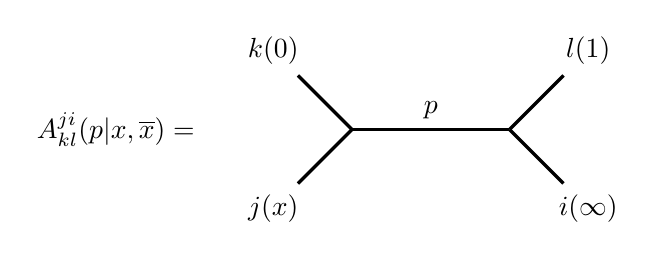
\begin{tikzpicture}[very thick]
	\node at (-1,1) (k) {$k (0)$};
	\node at (-1,-1) (j) {$j (x)$};
	\node at (3,1) (l) {$l (1)$};
	\node at (3,-1) (i) {$i (\infty)$};
	
	\node at (-3,0) {$A_{kl}^{ji}(p|x,\overline{x})=$};
	
	\draw (k) -- (0,0) ;
	\draw (j) -- (0,0);
	\draw (0,0) -- node[above] {$p$} ++ (2,0);
	\draw (2,0) -- (l);
	\draw (2,0) -- (i);
\end{tikzpicture}
\end{figure}

The partial wave factorizes in a holomorphic and antiholomorphic part, according to:
\begin{equation}
	A_{34}^{21}(p|x,\overline{x}) = \mathcal{F}_{34}^{21}(p|x)\overline{\mathcal{F}}_{34}^{21}(p|\overline{x}),
\end{equation}
we call these functions $\mathcal{F}$, the \emph{conformal blocks}. There is a recipe to compute these conformal blocks, even though it is a pain to compute these in practice. Physically speaking, these conformal blocks are the part in the four-point function that is fixed by conformal invariance. They depend on the anharmonic ratios via a series expansion. The remaining elements are the three-point coefficients, which are \emph{not} fixed by conformal invariance.

{\it Crossing symmetry and the conformal bootstrap}
What happens if we would choose instead of $z_4 = 0$, $z_1 = \infty$, $z_2 = 1$, $z_3 = x$ a different order of the fields? Following identities can be obtained relatively easy:
\begin{equation}
	G_{34}^{21}(x,\overline{x}) = G_{32}^{41}(1-x,1-\overline{x}),
\end{equation}
and
\begin{equation}
	G_{34}^{21}(x,\overline{x}) = \frac{1}{x^{2h_3}\overline{x}^{2\overline{h}_3}}G_{31}^{24}(1/x,1/\overline{x}).
\end{equation}
These identities are specific instances of the \emph{crossing symmetry} of the functions $G$. Explicitly we can write the first identity as
\begin{equation}
	\sum_p C_{21}^pC_{34}^p\mathcal{F}_{34}^{21}(p|x)\overline{\mathcal{F}}_{34}^{21}(p|\overline{x}) = \sum_q C_{41}^q C_{32}^q \mathcal{F}_{32}^{41}(p|1-x)\overline{\mathcal{F}}_{32}^{41}(p|1-\overline{x}),
\end{equation}
which has a aesthetically pleasing pictorial interpretation:
\begin{figure}
\centering
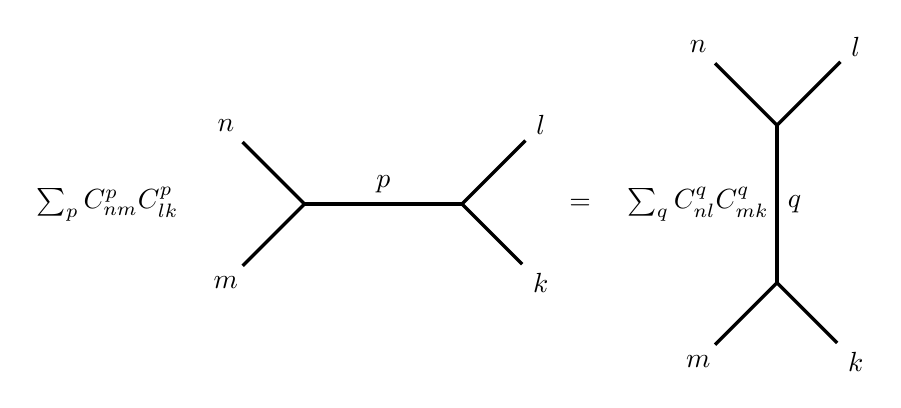
\begin{tikzpicture}[very thick]
\node at (-1,1) (k) {$n$};
\node at (-1,-1) (j) {$m$};
\node at (3,1) (l) {$l$};
\node at (3,-1) (i) {$k$};

\node at (-2.5,0) {$\sum_p C_{nm}^pC_{lk}^p$};

\draw (k) -- (0,0) ;
\draw (j) -- (0,0);
\draw (0,0) -- node[above] {$p$} ++ (2,0);
\draw (2,0) -- (l);
\draw (2,0) -- (i);

\node at (3.5,0) {$=$};

\begin{scope}[shift={(6,-1)}]
\node at (-1,-1) (m) {$m$};
\node at (1,-1) (k) {$k$};
\node at (-1,3) (n) {$n$};
\node at (1,3) (l) {$l$};

\node at (-1,1) {$\sum_q C_{nl}^qC_{mk}^q$};

\draw (m) -- (0,0) ;
\draw (k) -- (0,0);
\draw (0,0) -- node[right] {$q$} ++ (0,2);
\draw (0,2) -- (n);
\draw (0,2) -- (l);
\end{scope}
\end{tikzpicture}
\end{figure}
Crossing symmetry imposes $N^4$ constrains on the $N^3 + N$ parameters $C_{mn}^p$ and $h_p$. Exploiting crossing symmetry to compute these parameters is called \emph{conformal} bootstrap.

\section{Modular invariance}
Up until now we considered only CFTs on the infinite plane/Riemann sphere and at the exact fixed point. In that case the Hilbert space is a tensor product of a holomorphic and (completely decoupled) anti-holomorphic part. These parts don't interact and can this in principle describe completely different theories. In this section we will consider CFTs on the torus, still at the fixed point, in which case the two parts will need to be coupled in such a way that \emph{modular invariance} is preserved. This might seem somewhat ad hoc to define theories on a higher genus surface, but from a string theory point of view this is very natural. CFTs on higher genus surfaces describe higher order closed string scattering amplitudes. From a more stat mech point of view, a theory on a torus is simply a theory with periodic boundary conditions in both directions.
\subsection{Conformal field theory on the torus}
We will define the \emph{periods} of the lattice as linearly independent complex numbers $\omega_1,\omega_2$. The only dependence of the partition function can be on the \emph{modular} parameter $\tau=\omega_1/\omega_2$. As this is independent of the surface area and the absolute orientation of the periods.
{\bf The partition function}
In the operator formalism the partition function $Z$ and its dependence on $\tau$ stands central. We shall define the time and space direction to be the imaginary and real axis respectively. In that case:
\begin{equation}
	Z=\Tr\left(\exp(-\left\{H\Im\omega_2-iP\Re\omega_2\right\})\right),
\end{equation}
using
\begin{align}
	H &=  \frac{2\pi}{L}\left(L_0 + \bar L_0 -\frac{c}{12}\right)\\
	P &=  \frac{2\pi}{L}\left(L_0 - \bar L_0\right),
\end{align}
\footnote{{\color{red}Remark:} there is a misprint in the book: $P$ shouldn't have an $i$.} (the factor $c/12$ ensures the energy is zero in the infinite length case), we find:
\begin{equation}
	Z = \Tr(q^{L_0 - c/24}\bar q^{\bar L_0 -c/24}),
\end{equation}
where
\begin{align}
	q &= \exp(2\pi i\tau)\\
	\bar q &= \exp(-2\pi i\bar \tau).
\end{align}
We will see that the partition function will be a bilinear combination of characters.

{\bf Modular invarariance}
Suppose $\omega'_i$ define the same lattice, then necessarily:
\begin{equation}
\begin{pmatrix}
	\omega'_1\\
	\omega'_2
\end{pmatrix}
=
\begin{pmatrix}
	a & b\\
	c & d
\end{pmatrix}
\begin{pmatrix}
	\omega_1\\
	\omega_2
\end{pmatrix}.
\end{equation}
Where $\begin{pmatrix}
	a & b\\
	c & d
\end{pmatrix}\in SL(2,\mathbb{Z})$. The matrix has an integer inverse, and describes basis transformations that leave the surface area of the torus invariant.

Under a $SL(2,\mathbb{Z})$ transformation:
\begin{equation}
	\tau\mapsto\frac{a\tau + b}{c\tau +d},\qquad ad-bc=1.
\end{equation}
This leads to the modular group $SL(2,\mathbb{Z})/\mathbb{Z}_2=PSL(2,\mathbb{Z})$. Where the $\mathbb{Z}_2$ subgroup that is modded out corresponds to the symmetry $a,b,c,d\mapsto-a,-b,-c,-d$.


{\bf Generators and the fundamental domain}
The modular group is generated by:
\begin{align}
	&T:\tau\mapsto\tau +1,\qquad
	T =
	\begin{pmatrix}
		1 & 0\\
		1 & 1
	\end{pmatrix}\\
	&S:\tau\mapsto-\frac{1}{\tau},\qquad
	S =
	\begin{pmatrix}
		0 & -1\\
		1 & 0
	\end{pmatrix}.
\end{align}
And you can check $(ST)^3=S^2=-1$.\footnote{{\color{red}Remark:} there is a misprint in the book: $S$ is missing a minus sign and $(ST)^3=S^2=1$ should be $-1$.}

Geometrically, the modular group is generated by \emph{Dehn twists}: $T$ amounts to cutting the torus at fixed time and turning one of the ends $2\pi$ before gluing it back together. $U=TST$ does the same for fixed space. These are operators which are not smoothly connected to the identity.

A \emph{fundamental domain} $F$ is a part of the upper half complex plane that can be mapped to every other point of the complex plane by modular transformations. A convention for $F_0$ is:
\begin{equation}
	z\in F_0\quad\text{if}\quad
	\begin{cases}
		\Im z > 0, -\frac{1}{2}\leq \Re z\leq 0, \qquad|z|\geq 1\\
		\Im z > 0, 0< \Re z<\frac{1}{2},\qquad |z|\geq 1
	\end{cases}
\end{equation}
\subsection{The free boson on the torus}
Recall Dedekind's $\eta$ function:
\begin{equation}
	\eta(\tau) = q^{\frac{1}{24}}\prod_{n=1}^\infty (1-q^n).
\end{equation}
it can be shown that under modular transformations:
\begin{align}
	\eta(\tau+1) &= e^{i\pi/12}\eta(\tau)\\
	\eta(-1/\tau) &= \sqrt{-i\tau}\eta(\tau).
\end{align}
Without zero mode the boson partition function can be written as:
\begin{equation}
	Z_{\text{bos}}(\tau) = \frac{1}{(\Im\tau)^{1/2}|\eta(\tau)|^2}.
\end{equation}
This is a modular invariant combination of $\tau$ and can be obtained in the path-integral formalism by expanding the boson field in the eigenfunctions of the Laplacian and using $\zeta$-regularization.
\subsection{Free fermions on the Torus}
Fermion fields can be periodic or anti-periodic in two directions on the lattice:
\begin{align}
	\psi(z+\omega_1) &= e^{2\pi i \nu}\psi(z)\\
	\psi(z+\omega_2) &= e^{2\pi i u}\psi(z),
\end{align}
$\nu, u =0, \frac{1}{2}$, and we shall call the periodic boundary condition \emph{Ramond} and the anti-periodic boundary condition \emph{Neveu-Schwarz}. This leads to four different sectors. A set of boundary conditions is called a \emph{spin structure} for the fermion on the torus. Because $\psi$ and $\bar\psi$ decouple we can write:
\begin{equation}
	Z_{\nu, u} = |d_{\nu, u}|^2.
\end{equation}
A tedious computation leads to
\begin{align}
	d_{0,0} &= \frac{1}{\sqrt{2}}\Tr (-1)^F q^{L_0 - 1/48} = \frac{1}{\sqrt{2}}\Tr (-1)^Fq^{\sum_k kb_{-k}b_k+1/24},\\
	d_{0,\frac{1}{2}} &= \frac{1}{\sqrt{2}}\Tr  q^{L_0 - 1/48} = \frac{1}{\sqrt{2}}\Tr q^{\sum_k kb_{-k}b_k+1/24},\\
	d_{\frac{1}{2},0} &= \Tr (-1)^F q^{L_0 - 1/48} = \Tr (-1)^Fq^{\sum_k kb_{-k}b_k-1/48},\\
	d_{\frac{1}{2},\frac{1}{2}} &= \Tr q^{L_0 - 1/48} = \Tr q^{\sum_k kb_{-k}b_k-1/48},
\end{align}
or
\begin{align}
	d_{0,0} &= 0,\\
	d_{0,\frac{1}{2}} &= \sqrt{\frac{\theta_2(\tau)}{\eta(\tau)}},\\
	d_{\frac{1}{2},0} &= \sqrt{\frac{\theta_4(\tau)}{\eta(\tau)}},\\
	d_{\frac{1}{2},\frac{1}{2}} &= \sqrt{\frac{\theta_3(\tau)}{\eta(\tau)}}.
\end{align}
Remember the characters
\begin{equation}
	\chi_{(c,h)}(\tau) = \Tr q^{L_0 -c/24}.
\end{equation}
And the expressions for $L_0$:
\begin{align}
	L_0 &= \sum_{k>0} kb_{-k}b_k\qquad \left(k\in\mathbb{Z}+\frac{1}{2}\right),\\
	L_0 &= \sum_{k>0} kb_{-k}b_k + \frac{1}{16}\qquad \left(k\in\mathbb{Z}
	\right),
\end{align}
in the NS and R sectors.

Consider e.g. the NS sector. Since $L_0$ takes both half-integer and integer values, this character is the sum of at least two simple Virasoro characters. From the fact that $c=1/2$ we find that
\begin{align}
	\chi_{1,1} &= q^{-1/48}\frac{1}{2}\Tr(1+(-1)^F)q^{L_0}\\
	\chi_{2,1} &= q^{-1/48}\frac{1}{2}\Tr(1-(-1)^F)q^{L_0}.
\end{align}
Comparing with the partition function:
\begin{align}
	\chi_{1,1} &= \frac{1}{2}\left(d_{\frac{1}{2},\frac{1}{2}} + d_{\frac{1}{2},0}\right),\\
	\chi_{2,1} &= \frac{1}{2}\left(d_{\frac{1}{2},\frac{1}{2}} - d_{\frac{1}{2},0}\right).
\end{align}
Similarly for the R sector:
\begin{equation}
	\chi_{1,2} = \frac{1}{\sqrt{2}}d_{0,\frac{1}{2}}.
\end{equation}

From the modular transformation properties of the $d$'s, it follows there are two modular invariant partition functions: the one which only contains (R,R) and is zero and the one that combines the other sectors as:
\begin{align}
	Z &= Z_{\frac{1}{2},\frac{1}{2}} + Z_{0,\frac{1}{2}} + Z_{\frac{1}{2},0}\\
	&= \left|\frac{\theta_2}{\eta}\right| + \left|\frac{\theta_3}{\eta}\right| + \left|\frac{\theta_4}{\eta}\right|\\
	&= 2\left(|\chi_{1,1}|^2 + |\chi_{2,1}|^2 + |\chi_{1,2}|^2\right).
\end{align}
This is twice the partition function of the Ising model on the torus!



\section{FRS/Categorical construction of RCFT}
The mordern lanuage (probaly not the final lanuage of course) for RCFTs is the so-called category theory. The chiral symmetry of a RCFT is described by a (semisimple) modular tensor category $\mathcal{C}$. A full CFT requires the knowledge of how to combine the chiral and anti-chiral parts. Historically modular invariance has been utilized to construct a full CFT. However there exist non-physical modular invariant theories. The required part is a semisimple module category $\mathcal{M}$ over $\mathcal{C}$. Physically $\mathcal{M}$ contain information of how bulk fields interact with boundaries or more generally defects. Category theory provides a unified and beautiful lanuage of how bulk, boudary and defect fields interact, which compose a full CFT. 

\subsection{Chiral symmetry in RCFT}

\subsection{Verlinde lines in diagonal RCFT}

\subsection{Global symmetry and orbifold RCFT with discrete torsion}
With a given CFT $\mathcal{T}$ defined on $\mathcal{M}$ with a discrete global group symmetry $G$, it is possible to define a different CFT $\tilde{T} \sim T/G$ by gauging the global symmetry $G$~\cite{Douglas:aa,Gaberdiel_2000,Chang2019}. The orbifold theory $\tilde{T}$ then has a fusion category symmetry $\mathrm{Rep}(G)$. A symmetry operator or simple object in $\mathrm{Rep}(G)$ is labeled by $G$-representation. One-dimensional symmetry operators are invitable, while higher dimensional representations correspond to non-invitable symmetries. 

We first review the global symmetry $G$ in RCFT. Physically each symmetry operator $g$ can be represented by a line operator $\mathcal{L}_g$. We further require that $\mathcal{L}_g$ commutes with the chiral vertext algebra in RCFT, hence $\mathcal{L}_g$ is topological, which are denoted as topological defect lines (TDLs)~\footnote{There may exist conformal line operators which are not topological.}. Two symmetry operators can be fused into a new one, in which the fusion rule follows the multiplication of group elements. When fusing three operators, there are two different ways. These two fusion orders are related by a $F$-move, characterized by $\alpha(g,h,k)\,:\, 3$-cocycles $G^3 \rightarrow U(1)$ up to coboundaries. A non-trivival 3-cocycle means the global symmetry $G$ is anomalous in which the fusion of $\mathcal{L}_g$ not associative.

When $G$ is non-anomalous, we can construct orbifold theories. We start by inserting a symmetry projector $P := \frac{1}{|G|} \sum_{g \in G} \mathcal{L}_g$ in the partition function 
\begin{equation}
	\begin{aligned}
		Z = \mathrm{Tr}\left( P\,q^{L_0} \bar{q}^{\bar{L}_0} \right).
	\end{aligned}
\end{equation}
However, this theory is usually not modular invariant, since a modular transformation can modifies the symmetry action in the time direction and generate different terms. One needs to consider the so-called twisted sectors in the Hilbert space $\mathcal{H}_h$ to construct a modular invariant theory. This twisted sector $\mathcal{H}_h$ is difind according to
\begin{equation}
	\phi(e^{2\pi i}z,e^{-2\pi i}\bar{z}) = \mathcal{L}_h \circ \phi(z,\bar{z}).
\end{equation}
Now after symmetrilization, one writes down the orbifold theory
\begin{equation}
	\begin{aligned}
		Z(q,\bar{q}) = \frac{1}{|G|}\,\sum_{[g,h]=0}\mathrm{Tr}_{\mathcal{H}_h}\left( \mathcal{L}_g \, q^{L_0} \bar{q}^{\bar{L}_0} \right).
	\end{aligned}
\end{equation}

For a given symmetry group $G$, there may exist different orbifold ways. It turns out one can use the second cohomology group $H^2(G,U(1))$ to classify orbifolds. This is known as discrete torsion in the literature. Specifically one can use $\epsilon(g,h)$ to characterize each orbifold theory
\begin{equation}
	\begin{aligned}
		Z(q,\bar{q}) = \frac{1}{|G|} \, \sum_{[g,h]=0} \epsilon(g,h) \, \mathrm{Tr}_{\mathcal{H}_h}\left( \mathcal{L}_g \, q^{L_0} \bar{q}^{\bar{L}_0} \right),
	\end{aligned}
\end{equation}
where $\epsilon(g,h) := \nu(g,h)/\nu(h,g)$ with $\nu(g_1,g_2)$ being two cocycles. The symmetry projector becomes $P_h := \frac{1}{|G|}\sum_g \epsilon(g,h)\,\mathcal{L}_g$. 

\subsection{Duality TDL and Self-dual orbifold}

\subsection{Topological defects in Ising CFT}
Besides the closed manifolds, CFTs can also be defined on manifols with boundaries, or defects in more general setting. A boundary can be understood a special defect between a CFT and a trivial CFT with a central charge $c=0$. On the other hand a defect between CFT1 and CFT2 can be regarded as a boundary of stacking the two CFTs using the folding trick. It is natural to require the conformal symmetry still holds at boundaries and defects. For a boundary state $\vert a \rangle$ this means 
\begin{equation}
	\left ( L_n - \bar{L}_{-n} \right ) \vert a \rangle = 0.
\end{equation}
For a defect $O_\alpha$ it requires
\begin{equation}
	\left[ L_n - \bar{L}_{-n},\, O_\alpha \right] = 0.
\end{equation}
Usually we require stronger constraint for the conformal defects 
\begin{equation}
	\begin{aligned}
		\left[ L_n,\, O_\alpha \right] = 0 \\
		\left[ \bar{L}_{n},\, O_\alpha \right] = 0
	\end{aligned}
\end{equation}
which are now called topological defects. They correspond to the topological aspects of CFT and serve the role of intertwiners between conformal boundaries. Since the topological defects commute with Virasoro generators, they can be viewed as genearlized symmetries. 

Let's start with a simple example -- the Ising CFT $\mathcal{M}(4,3)$. There are three conformal boundaries/topological defects in Ising CFT which are labeled by primaries. Two defects can be fused into other defects when put close to each other. As a result their fusion forms a fusion algebra. In Ising CFT, the fusion algebra of defects is the same as that of primaries. This is true for all A-type minimal models. 

\subsection{Boundary states}

\section{Other topics}
\subsection{Boundary conformal field theory}
CFT can also be defined in a manifold with boundaries, in which the nice local properties are still applied from the CFT defined on a plane. A boundary conformal field theory (BCFT) is a CFT defined on a two dimension manifold with one dimension boundaries. It is important theoretical tool in the study of surface critical behavior, defects and open string theories. Note that one can also consider extended symmetry in a CFT, so that the Virasoro algebra is a subalgebra of the extended symmetry. The corresponding boundary condition (resp. boudary state) in the open (resp. closed) sector should also respect the extended algebra. It was shown than there are also symmetry-breaking boundary conditions which only respect the conformal symmetry. Here we only discuss conformal symmetry. 

{\bf BCFT in the open sector}
We define a BCFT on a cylinder with two boundaries $B_a$ and $B_b$. The complex coordinate is denoted by $\omega = \tau + i \sigma$, where we identify the time $\tau$ ($\tau \in [0,2\pi t]$) direction to be periodic and space $\sigma$ ($\sigma \in [0,\pi]$) to be open. When the time direction range is unbounded $t\rightarrow\infty$, the cylinder becomes a strip. Since the Hamiltonian $H_{ab}$ generating time evolution is defined at a fixed time with two boundaries, the whole Hilbert space is constrained by the boundary conditions at $B_a$ and $B_b$. To apply the powerful conformal symmetry to the strip, one can apply the conformal mapping $z = e^\omega = e^\tau e^{i\sigma}$ to relate the strip to the upper half-plane. The energy-momentum tensor has to be real at the boundary, so that
\begin{equation} \label{Eq_T_open}
    T(z) - \bar{T}(\bar{z})\vert_{\sigma=0,\pi} = 0
\end{equation}
or in terms of Laurent series 
\begin{equation}
    \sum_n L_n z^{-n-2} - \sum_n \bar{L}_n \bar{z}^{-n-2}\vert_{\sigma=0,\pi} = 0. 
\end{equation}
One then finds the two Virasoro algebra now reduces to a single algebra under the constraint $L_n = \bar{L}_n$. This is naturally satisfied if one identifies the antiholomorphic coordinate $\bar{z}$ in the upper half-plane to be the holomorphic one $z^*$ in the lower half-plane. As a result, a BCFT defined on a strip is mapped to a chiral CFT defined on a plane. 

With this identification, one can express operators defined on a cylinder in terms of those defined on a plane. The Hamiltonian operator is 
\begin{equation}
    H_{ab} = L_0 - \frac{c}{24}. 
\end{equation}
The partition function can also be written down 
\begin{equation}
    Z_{ab} = \mathrm{Tr}\,\left( e^{-2\pi t\, H_{ab}}\right) = \mathrm{Tr}\,\left( q^{L_0-c/24}\right),
\end{equation}
where $q=e^{\pi i\, \tau_{open}}$ and the modular parameter $\tau_{open} = i\,t$. As stated above, the Hilbert space is determined by the boundaries $B_{a/b}$. A conformal family $[\phi_{h}(z)]$ appearing in the chiral theory should be consistent with the boundary conditions. The partition function can be written as 
\begin{equation}
    Z_{ab} = \sum_h n_{ab}^h\, \chi_h(q)
\end{equation}
where the non-negative integer $n_{ab}^h$ selects the conformal families appearing in the theory and the character $\chi_h(q) = \mathrm{Tr}_h\,\left( q^{L_0-c/24}\right)$.

{\bf BCFT in the closed sector}
In the open sector the time direction is chosen to be periodic. Meanwhile one has the freedom to define the space $\sigma$ ($\sigma \in [0,2\pi]$) direction to be periodic and time $\tau$ to be open ($\tau \in [0,2\pi\,l]$), which is the closed sector. The calculation of partition function becomes a time evolution
\begin{equation}
    Z_{ab} = \langle a \vert e^{-2\pi l H} \vert b \rangle = \langle a \vert e^{-2\pi l (L_0 + \bar{L}_0 -c/12)} \vert b \rangle,
\end{equation}
where the time evolution operator $H$ defined on a cylinder is the dilation operator on the plane $H = L_0 + \bar{L}_0 - c/12$. 

The physical constraint Eq.~\ref{Eq_T_open} in the closed sector now becomes 
\begin{equation}
    z^2 T(z) - \bar{z}^2 \bar{T}(\bar{z})\vert_{\tau=0,2\pi l} = 0.
\end{equation}
Note that due to the choice of time direction, the boundary condition is a constraint to the boundary state $\vert a \rangle$ and $\vert b\rangle$. In terms of Laurent modes, this is
\begin{equation}
    \begin{split}
        \left(L_n - \bar{L}_{-n}\right) \vert a \rangle = 0.  
    \end{split}
\end{equation}
The basis state of the solution is the so-called Ishibashi state
\begin{equation}
    \vert h \rangle\rangle = \sum_n \vert h,n\rangle \otimes U\overline{\vert h,n\rangle},
\end{equation}
where $U$ is an anti-unitary operator which commutes with Virasoro generators, $h$ denotes a conformal family $\phi_h$. If there are a finite number representations of the Virasoro algebar in the theory, one can construct physical boundary states, the Cardy states, in terms of the Ishibashi states
\begin{equation}
    \vert a \rangle = \sum_h c_a^h\, \vert h \rangle \rangle. 
\end{equation}
The partition function $Z_{ab}$ then reads
\begin{equation}
    Z_{ab} = \sum_h \left(c_a^h\right)^* c_b^h\, \chi_h(\tilde{q})
\end{equation}
where $\tilde{q} = e^{2\pi i \tau_{closed}}$ with the modular parameter $\tau_{closed} = 2i\,l = i/t$.

{\bf Open-closed BCFT duality}
The open and closed sector theories are essentially describing the same $Z_{ab}$. They are related through a modular transformation of the modular parameter $\tau \rightarrow -1/\tau$ which exchange the role of space and time. The characters are related by a $S$ matrix 
\begin{equation}
    \chi_j(\tilde{q}) = \sum_i S^i_j\, \chi_i(q).
\end{equation}
This gives the Cardy conditions to the BCFT
\begin{equation}
\begin{split}
    & n_{ab}^h = \sum_i \left(c_a^i\right)^* c_b^i\, S_i^h \\
    & \left(c_a^h\right)^* c_b^h = \sum_i n_{ab}^i S^h_i.  
\end{split}
\end{equation}
For minimal models the Cardy states can be constructed by requiring
\begin{equation}
\begin{split}
    c_a^h &= S_a^h / \sqrt{S^h_0} \\
    n_{ab}^h &= \sum_i \frac{\left(S_a^i\right)^* S_b^i S_h^i}{S_0^i}.
\end{split}
\end{equation}
Comparing with the Verlinde formula, one can identify the coefficient $n_{ab}^h$ is the same as the fusion multiplicities $N_{ab}^h$. It is now clear that the conformal families appearing in the open sector theory is determined by the fusion of the primaries representing the Cardy states in the closed sector. 

\subsection{Bosonization}
In the discussion of free compact boson theory, we have seen the vertex operator $V_1 = :e^{i\phi(z,\bar{z})}:$ has the same scaling dimension as a fermion operator and more importantly the free complex fermion and and the free compact boson (with a radius $R=1$) share the same partiton function. These facts indicate that the fermion and boson theories are dual to each other. 

{\bf Bosonization dictonary for free fermions---}
With the chiral mass center introduced above the chiral part of the compact boson field $X(z,\bar{z}) = \phi(z) + \bar{\phi}(\bar{z})$ can be expanded in terms of current operators. Recall that the two-point correlation of free boson. The current operator can be defind as 
\begin{equation}
	J(z) = i\sqrt{\frac{2}{K}}\partial \phi (z).
\end{equation} 
So that the chiral/anti-chiral part of the free compact boson can be written as 
\begin{equation}
	\begin{split}
		\phi(z) &= \sqrt{\frac{K}{2}}\left(\phi_0 -i\,j_0\,\mathrm{ln}\,z + i\,\sum_{n\neq0} \frac{1}{n}\,j_n\,z^{-n}\right) \\
		\bar{\phi}(\bar{z}) &= \sqrt{\frac{K}{2}} \left(\bar{\phi}_0 -i\,\bar{j}_0\,\ln \,\bar{z} + i\,\sum_{n\neq0} \frac{1}{n}\,\bar{j}_n\,{\bar{z}}^{-n}\right).
	\end{split}
\end{equation} 
The zero mode of the current operator is quantitized to be 
\begin{equation}
	\begin{aligned}
		j_0 &= \frac{1}{\sqrt{2}} \left( \frac{\sqrt{K}m}{R} + \frac{R}{\sqrt{K}n} \right) \\
		\bar{j}_0 &= \frac{1}{\sqrt{2}} \left( \frac{\sqrt{K}m}{R} - \frac{R}{\sqrt{K}n} \right)
	\end{aligned}
\end{equation}
One can also introduce its dual field $\tilde{X} := \phi(z) - \bar{\phi}(z)$. It is compactified on a circle with a radius $K/R$. This indicates that there are two $U(1)$ symmetry in the free compact boson theory, which correspond to $X$ and $\bar{X}$ fields respectively.

Now we are ready to bosonize the fermion fields with the vertex operators
\begin{equation}
	\begin{split}
		&\psi(z) \sim e^{i\sqrt{\frac{2}{K}}\,\phi(z)} \\
		&\bar{\psi}(\bar{z}) \sim e^{i\sqrt{\frac{2}{K}}\,\bar{\phi}(\bar{z})}.
	\end{split}
\end{equation}




\if_false:
{\bf Dual field approach}\\
Recall the compact boson compactified on a $2\pi\,R$ circle (we have chosen $K=2$) has the mode expansion
\begin{equation}
	\begin{split}
		X(z,\bar{z}) = x_0 -i\left(j_0\,\mathrm{ln}\,z + \bar{j}_0\,\ln\,\bar{z}\right) + i\,\sum_{n\neq0} \left(\frac{1}{n}\,j_n\,z^{-n}+\frac{1}{n}\,\bar{j}_n\,\bar{z}^{-n}\right).
	\end{split}
\end{equation} 
Its conjugate momentum field $\pi(z,\bar{z}):=\frac{\partial\,L}{\partial\partial_tX(z,\bar{z}))} = \frac{1}{4\pi}\,i\,\partial_\tau X$ can be written as
\begin{equation}
	\pi(z,\bar{z}) = \frac{1}{4\pi} \left(i\partial X + i\bar{\partial} X\right) = \frac{1}{4\pi} \left(j(z) + \bar{j}(\bar{z})\right) = \frac{1}{4\pi} \partial_t X(z,\bar{z}),
\end{equation}
which is consistent with the quantization condition $[X(\tau,\sigma),\pi (\tau,\sigma')] = i\,\delta(\sigma-\sigma')$. Note the communication relation $[x_0,\,\left(j_0+\bar{j}_0\right)/2] = i$ has been assumed here. 

It is usually convenient to introduce the dual field of $X(z,\bar{z})$
\begin{equation}
	\begin{split}
		\theta(z,\bar{z}) = x_0 -i\left(j_0\,\mathrm{ln}\,z - \bar{j}_0\,\mathrm{ln}\,\bar{z}\right) + i\,\sum_{n\neq0} \left(\frac{1}{n}\,j_n\,z^{-n}-\frac{1}{n}\,\bar{j}_n\,\bar{z}^{-n}\right).
	\end{split}
\end{equation} 
One finds that 
\begin{equation}
	\begin{split}
		j(z) &= i\partial\theta(z,\bar{z}) \\
		\bar{j}(\bar{z}) &= -i\bar{\partial}\theta(z,\bar{z})\\
		j+\bar{j} &= i\left(\partial\theta-\bar{\partial}\theta\right) = \partial_\sigma \theta(z,\bar{z}) = \partial_t X(z,\bar{z}) \\
		j-\bar{j} &= i\left(\partial\theta+\bar{\partial}\theta\right) = \partial_t \theta(z,\bar{z}) = \partial_\sigma X(z,\bar{z})
	\end{split}
\end{equation}
It is clear that the dual field $\theta(z,\bar{z})$ is compactified on a radius $\rho = 2/R$ circle. This means the duality above can be formulated as $R \rightarrow 2/R$. Now one can try to express the fermion operators in terms of $X$ and $\theta$. However, there are two difficulties using such an approach. 

First, when one tries to rewritte the action in terms $\theta$ field, there is an extra minus sign in the action both in Minkoswki and Euclidean space. To ensure the convergence of the Euclidean space action, one has to use a different analytic continuuation $\tau = -i\,t$, which is not consistent with our convention.

Second, the zero mode is not consistent with the quantization condition. This can be easily seen in the communicator $\left[x_0,\,\left(j_0+\bar{j}_0\right)\right] \neq i$. This contraction actually can be cured by introducing the chiral mass center $x_0 = \phi_0 + \bar{\phi}_0$ which satisfies
\begin{equation}
	\begin{split}
		&\left[\phi_0,j_0\right] = i\\
		&\left[\bar{\phi}_0,\bar{j}_0\right] = i\\
		&\left[\phi_0,\bar{\phi}_0\right] = 0 \\
		&\left[x_0,\left(j_0+\bar{j}_0\right)/2\right] = i.
	\end{split}
\end{equation}

{\bf Chiral field approach}\\
With the chiral mass center introduced above the compact boson field can be written as 
\begin{equation}
	\begin{split}
		X(z,\bar{z}) &= \phi(z) + \bar{\phi}(\bar{z}) \\
		\phi(z) &= \phi_0 -i\,j_0\,\mathrm{ln}\,z + i\,\sum_{n\neq0} \frac{1}{n}\,j_n\,z^{-n} \\
		\bar{\phi}(\bar{z}) &= \bar{\phi}_0 -i\,\bar{j}_0\,\mathrm{ln}\,\bar{z} + i\,\sum_{n\neq0} \frac{1}{n}\,\bar{j}_n\,\bar{z}^{-n}.
	\end{split}
\end{equation} 
Now we are ready to bosonize the fermion fields with the vertex operators
\begin{equation}
	\begin{split}
		&\psi(z) \sim \mathcal{N}\left(e^{i\phi(z)}\right) \\
		&\bar{\psi}(\bar{z}) \sim \mathcal{N}\left(e^{i\bar{\phi}(\bar{z})}\right)
	\end{split}
\end{equation}


\fi
\appendix

\section{Central extensions of Lie algebras}
In this section $\mathfrak{g},\mathfrak{h},...$ denote (possibly infinite) Lie algebras over some field $\mathbb{K} = \mathbb{R}, \mathbb{C}$. This section is mainly based on Wikipedia and~\cite{Schottenloher}.


\subsection{Extensions}
{\bf Definition:} A \emph{Lie algebra extension} is a short exact sequence of Lie algebras:
\begin{equation}
	\mathfrak{h}\overset{\iota}{\rightarrow}\mathfrak{e}\overset{\pi}{\rightarrow}\mathfrak{g}.
\end{equation}
One calls $\mathfrak{e}$ an extension of $\mathfrak{g}$ by $\mathfrak{h}$. By exactness of the sequence one has $\mathfrak{g}\cong\mathfrak{e}\slash\Ima\iota$.\\

{\bf Definition:} A \emph{central extension} is an extension $\mathfrak{e}$ of $\mathfrak{g}$ by $\mathfrak{h}$, such that $\Ima \iota$ is contained in the center of $\mathfrak{e}$, $\iota(\mathfrak{h})\subseteq Z(\mathfrak{e})$.\\

Notice that for a central extension $\mathfrak{h}$ is necessarily abelian. We now introduce a notion of trivial central extensions as follows:

{\bf Definition:} A Lie algebra extension
\begin{equation}
	\mathfrak{h}\overset{\iota}{\rightarrow}\mathfrak{e}\overset{\pi}{\rightarrow}\mathfrak{g}
\end{equation}
\emph{splits} if there exists a Lie algebra morphism $\beta: \mathfrak{g}\mapsto\mathfrak{e}$ such that $\pi\circ\beta = \text{id}_{\mathfrak{e}}$. $\beta$ is called a splitting map.\\

A central extension
\begin{equation}
	\mathfrak{h}\overset{\iota}{\rightarrow}\mathfrak{e}\overset{\pi}{\rightarrow}\mathfrak{g}.
\end{equation}
that splits is trivial in the sense that it is equivalent\footnote{To do: introduce the notion of equivalent extensions.} to one where $\mathfrak{e}\cong\mathfrak{g}\oplus\mathfrak{h}$.\\

Let us now consider a central extension and a map (not necesserily a Lie algebra homomorphism) $\beta:\mathfrak{g}\rightarrow\mathfrak{e}$ such that $\pi\circ\beta = \text{id}_{\mathfrak{e}}$. From this map construct
$\Theta: \mathfrak{g}\times\mathfrak{g}\rightarrow\mathfrak{h}$ as follows:
\begin{equation}
	\Theta(x,y) := \left[\Theta(x),\Theta(y)\right] - \Theta\left([x,y]\right).
\end{equation}
This map is:
\begin{enumerate}
	\item \label{prop:antisym} Antisymmetric.
	\item \label{prop:bilinear} Bilinear.
	\item \label{prop:Jacobi} Satisfies $\Theta(x,[y,z]) + \Theta(y,[z,x]) + \Theta(z,[x,y]) = 0$.
\end{enumerate}
Given $\Theta$ one can now show that there is an isomorphism between the vector spaces $\mathfrak{e}\cong\mathfrak{g}\oplus\mathfrak{h}$ that is given by:
\begin{equation}
	\Psi:\mathfrak{g}\oplus\mathfrak{h}\mapsto\mathfrak{e}:(x,y)\mapsto\beta(x) + y.
\end{equation}
A Lie bracket on $\mathfrak{g}\oplus\mathfrak{h}$ is given by:
\begin{equation}
	[x\oplus z, y\oplus z']_{\mathfrak{e}} := [x,y]_\mathfrak{g} + \Theta(x,y).
\end{equation}

{\bf Lemma:} In the above construction $\beta$ is a splitting map if and only if
\begin{equation}
	\Theta(x,y) = \mu([x,y]),
\end{equation}
for some $\mu\in\text{Hom}(\mathfrak{g},\mathfrak{h})$.\\

Now comes the classification of central extensions of Lie algebras:\\

{\bf Theorem:} Every central extension comes from a map $\Theta$ that satisfies the above properties (\ref{prop:antisym}-\ref{prop:Jacobi}). Conversely, every central extension gives rise to a map $\Theta$ that satisfies the above properties (\ref{prop:antisym}-\ref{prop:Jacobi}).

\subsection{Lie algebra cohomology}
The classification of Lie algebra extensions is very satisfying. It smells a lot like a cohomological classification. Indeed, the extensions are classified by functions depending on two variables satisfying the condition (\ref{prop:Jacobi}) that is exactly the one needed to fulfill the Jacobi identity of the central extension. Moreover, the central extension is trivial if the \emph{2-cocycle} $\Theta$ is trivial in the following sense: $\Theta(x,y) = \mu([x,y])$. This is reminiscent of considering 2-cocycles to be trivial if they are equal to a coboundary. Let us put this on a bit more rigorous footing.\\

{\bf Definitions:}
\begin{enumerate}
	\item $Z^2(\mathfrak{g},\mathfrak{h}) = \left\{\Theta\in\Lambda^2(\mathfrak{g},\mathfrak{h})|\Theta:(\ref{prop:Jacobi})\right\}$.
	\item $B^2(\mathfrak{g},\mathfrak{h})=\left\{\Theta:\mathfrak{g}\times\mathfrak{g}\mapsto\mathfrak{h}|\exists\mu\in\text{Hom}(\mathfrak{g},\mathfrak{h}):\Theta(-,-)=\mu([-,-])\right\}$.
	\item $H^2(\mathfrak{g},\mathfrak{h}):=Z^2(\mathfrak{g},\mathfrak{h})/B^2(\mathfrak{g},\mathfrak{h})$.
\end{enumerate}
$H^2$ is of course called the second cohomology group. We thus obtain the following reformulation of the classification of central extensions:\\

{\bf Theorem:} The equivalence classes of central extensions
\begin{equation}
	\mathfrak{h}\overset{\iota}{\rightarrow}\mathfrak{e}\overset{\pi}{\rightarrow}\mathfrak{g}
\end{equation}
are in one-to-one correspondence with the elements of $H^2(\mathfrak{g},\mathfrak{h})$.\\

For completeness, let us introduce a notion of cochain complexes for Lie algebras. A cochain $f$ is a alternating multilinear map $f$:
\begin{equation}
	f:\Lambda^n \mathfrak{g} \mapsto \mathfrak{h}.
\end{equation}
Here, $\mathfrak{h}$ is considered a $\mathfrak{g}$-module or -representation.

The differential of an $n$-cochain is given by
\begin{equation}
\begin{aligned}
	(d f)\left(x_1, \ldots, x_{n+1}\right) =
	&\sum_i     (-1)^{i+1}x_i\, f\left(x_1, \ldots, \hat x_i, \ldots, x_{n+1}\right) + \\
	&\sum_{i<j} (-1)^{i+j}      f\left(\left[x_i, x_j\right], x_1, \ldots, \hat x_i, \ldots, \hat x_j, \ldots, x_{n+1}\right)\, ,
\end{aligned}
\end{equation}

so for example, with trivial action we obtain
\begin{equation}
	(df)(x_1,x_2) = f([x_1,x_2]),
\end{equation}
and
\begin{equation}
\begin{aligned}
	(df)(x_1,x_2,x_3) &= -f([x_1,x_2],x_3) + f([x_1,x_3],x_2) - f([x_2,x_3],x_1)\\
	&= -f([x_1,x_2],x_3) - f([x_3,x_1],x_2) - f([x_2,x_3],x_1)\\
	&= f(x_3,[x_1,x_2]) + f(x_2,[x_3,x_1]) + f(x_1,[x_2,x_3]).
\end{aligned}
\end{equation}
So clearly, $Z^2(\mathfrak{g},\mathfrak{h})$ defined above is the group of 2-cocycles satisfying $d\Theta=0$ and $B^2(\mathfrak{g},\mathfrak{h})$ the set of coboundaries: $\Theta = d\mu$.
\bibliography{refs.bib}

\nolinenumbers

\end{document}
